\section{Estimateurs d'environnement}
\label{sec:env}
% =====================================================================

Les deux estimateurs sont évalués sur la \emph{boîte périodique entière}, et sur le même ensemble de $N_r = N_g$ points aléatoires uniformes (graine fixe, tirés dans le cube unité et remis à l'échelle de la boîte, de sorte que les points aléatoires sont identiques dans toutes les cosmologies à la mise à l'échelle AP près).

\subsection{ASTRA split}

Les galaxies et les points aléatoires sont réunis en un seul catalogue et triangulés selon Delaunay. Pour chaque point (galaxie ou aléatoire), avec $N_{\rm data}$ et $N_{\rm rand}$ les nombres de galaxies et d'aléatoires parmi ses voisins de Delaunay,
\begin{equation}
r = \frac{N_{\rm data}-N_{\rm rand}}{N_{\rm data}+N_{\rm rand}} \in [-1,1].
\label{eq:astra_r}
\end{equation}
Un point entouré de galaxies ($r\to1$) se trouve dans une région dense, un point entouré d'aléatoires ($r\to-1$) dans une région sous-dense. Dans la classification ASTRA originale \cite{ASTRA}, des seuils sur $r$ définissent les vides, feuillets, filaments et nœuds ; ici nous utilisons $r$ comme variable d'environnement continue. La triangulation est calculée indépendamment dans chaque sous-volume (Section~\ref{sec:clustering}) sur une région étendue de $30\Mpch$ de chaque côté, avec un repliement périodique à travers les faces de la boîte, et $r$ n'est conservé que pour les points à l'intérieur du sous-volume. Cela supprime les effets de bord d'une triangulation non périodique (voisins manquants, simplexes de bord allongés). La séparation moyenne entre points du catalogue joint est $\simeq10\Mpch$, de sorte que l'extension contient plusieurs couches de voisins (convergence dans la Section~\ref{sec:robustness}).

\subsection{Density split}

Comme référence, nous utilisons le density split standard \cite{Paillas2023}. Les galaxies sont affectées à un maillage périodique de cellules de $5\Mpch$ par un schéma nuage-dans-la-cellule (CIC), le champ de surdensité est lissé par un noyau gaussien de rayon $R_s=10\Mpch$ par FFT, et le contraste de densité lissé $\delta_R$ est lu (CIC) à la position de chaque galaxie et de chaque point aléatoire.

\subsection{Quartiles d'environnement}

Pour chaque méthode, chaque sous-volume et chaque population, les points sont classés selon leur valeur d'environnement ($r$ ou $\delta_R$) et répartis en quatre quartiles de taille exactement égale, de Q1 (le plus sous-dense) à Q4 (le plus surdense). Comme $r$ est un rapport de petits entiers, de nombreux points partagent la même valeur ; les égalités sont départagées au hasard. Nous considérons deux populations, classées séparément de sorte que les seuils de l'une ne dépendent pas de l'autre :
\begin{itemize}
\item \textbf{quartiles aléatoires} : les points aléatoires classés selon leur environnement, les points de requête du density split, échantillonnant les environnements par volume ;
\item \textbf{quartiles de galaxies} : les galaxies classées selon leur propre environnement, échantillonnant les environnements par masse.
\end{itemize}

\subsection{Classes de toile cosmique et raison de l'usage des quartiles}
\label{sec:classes_def}

ASTRA a été conçu pour classer les points en quatre classes de toile cosmique avec des seuils fixes sur $r$ \cite{ASTRA} : vides ($r\le-0.9$), feuillets ($-0.9<r\le0$), filaments ($0<r\le0.9$) et nœuds ($r>0.9$). Nous utilisons exactement la définition de l'implémentation de référence (Éq.~\ref{eq:astra_r} avec $N_r=N_g$, $r$ issu d'un seul catalogue aléatoire, ces seuils). Sur le catalogue fiduciel de type DESI, les classes sont extrêmement déséquilibrées (Figure~\ref{fig:map}) : 0.25\% des points aléatoires sont des vides, 65\% des feuillets, 34\% des filaments et 0.05\% des nœuds ; pour les galaxies 0.07\%, 49\%, 51\% et 0.3\%. Dans Quijote, 0.7\%, 72\%, 27\% et 0\% des points aléatoires. En pratique, la classification se réduit à \emph{deux classes dominantes}, feuillets et filaments, c'est-à-dire à une coupure de $r$ à zéro ; les vides et les nœuds contiennent quelques centaines de points par sous-volume, trop peu pour des mesures de clustering précises (Figure~\ref{fig:classes_mp}). Ce déséquilibre a motivé l'usage de quartiles de $r$ de taille égale dans l'analyse principale, qui conservent le classement des environnements par ASTRA tout en donnant à chaque environnement le même poids statistique, comme dans le density split.

L'article ASTRA rapporte 7--11\% de points aléatoires dans les vides \cite{ASTRA}, contre 0.25--0.7\% ici. Ses échantillons sont 11 à 73 fois plus denses que nos LRG (densités numériques de $1.7\times10^{-3}$ à $1.1\times10^{-2}\,{\rm Mpc}^{-3}$, contre $1.5\times10^{-4}\,{\rm Mpc}^{-3}$). Les fractions ne sont pas fixées par la seule densité (les halos de Quijote, dix fois plus épars que les LRG mais plus fortement corrélés, ont davantage de vides), mais par le contraste de densité du champ de traceurs à l'échelle de la séparation moyenne entre points. C'est une autre manifestation de l'échelle adaptative d'ASTRA (Section~\ref{sec:robustness}) : des seuils fixes sur $r$ ne sélectionnent pas les mêmes environnements dans des échantillons de densité et de biais différents, alors que les quantiles de $r$ définissent des environnements comparables.


\begin{figure*}[!tp]
\centering
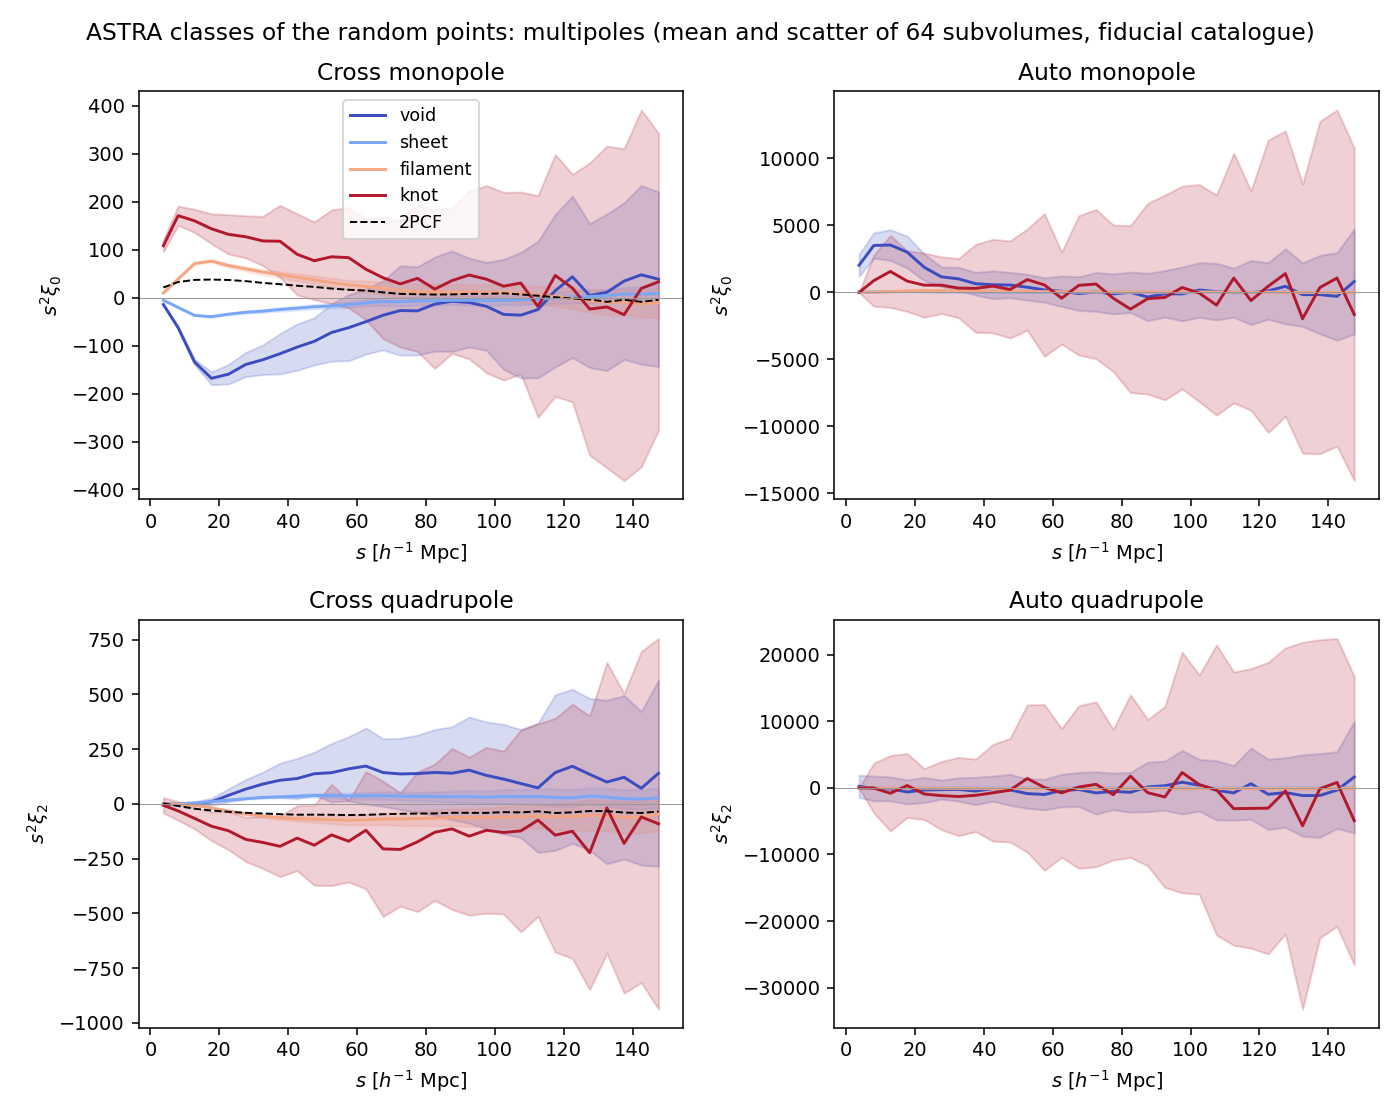
\includegraphics[width=\textwidth]{classes_abacus_multipoles.png}
\caption{Monopôle (haut) et quadrupôle (bas) des classes ASTRA des points aléatoires sur le catalogue fiduciel : cross-corrélation avec les galaxies (gauche) et auto-corrélation (centre) des feuillets et des filaments, et cross-corrélation des vides et des nœuds (droite, autre échelle). Lignes et bandes : moyenne et dispersion à $1\sigma$ des 64 sous-volumes ; tirets : 2PCF. Les filaments se comportent comme le quartile surdense Q4 et les feuillets comme le quartile sous-dense Q1 ; les vides et les nœuds ne contiennent que $\sim150$ et $\sim30$ points aléatoires par sous-volume, d'où leur grande dispersion.}
\label{fig:classes_mp}
\end{figure*}

\subsection{Comparaison des deux classifications}

La Figure~\ref{fig:env} compare les deux estimateurs sur le catalogue fiduciel. Ils sont fortement mais pas parfaitement corrélés : la corrélation de rang de Spearman entre $r$ et $\delta_R$ est $0.719\pm0.005$ pour les points aléatoires et $0.713\pm0.005$ pour les galaxies (dispersion sur les sous-volumes). Les quartiles extrêmes sont les plus cohérents : 63\% des points aléatoires du Q1 (Q4) d'ASTRA sont aussi dans le Q1 (Q4) du density split, alors que les quartiles intermédiaires sont largement mélangés, et moins de 2\% des points passent d'un extrême à l'autre. ASTRA identifie les mêmes structures à grande échelle que le density split mais redistribue de nombreux points (Figure~\ref{fig:map}), comme attendu d'une échelle adaptative plutôt que fixe. Les distributions de $r$ et de $\delta_R$ par quartile sont montrées dans la Figure~\ref{fig:envhist}.

\paragraph{Réponse à la cosmologie.} La Figure~\ref{fig:response} montre comment l'environnement moyen de chaque quartile des halos de Quijote se décale lorsqu'un paramètre cosmologique varie, en unités de sa dispersion entre réalisations. Le contraste $\delta_R$ du density split répond fortement (jusqu'à $7\sigma$ pour $\sigma_8$), de façon antisymétrique pour les variations $\pm$ ; la valeur ASTRA $r$ bouge à peine ($<1\sigma$). C'est attendu : $r$ est normalisé localement par les points aléatoires et est presque insensible à l'amplitude globale du champ. L'information cosmologique de l'ASTRA split réside donc dans le clustering de ses environnements plutôt que dans les valeurs de $r$.

\begin{figure*}[!tp]
\centering
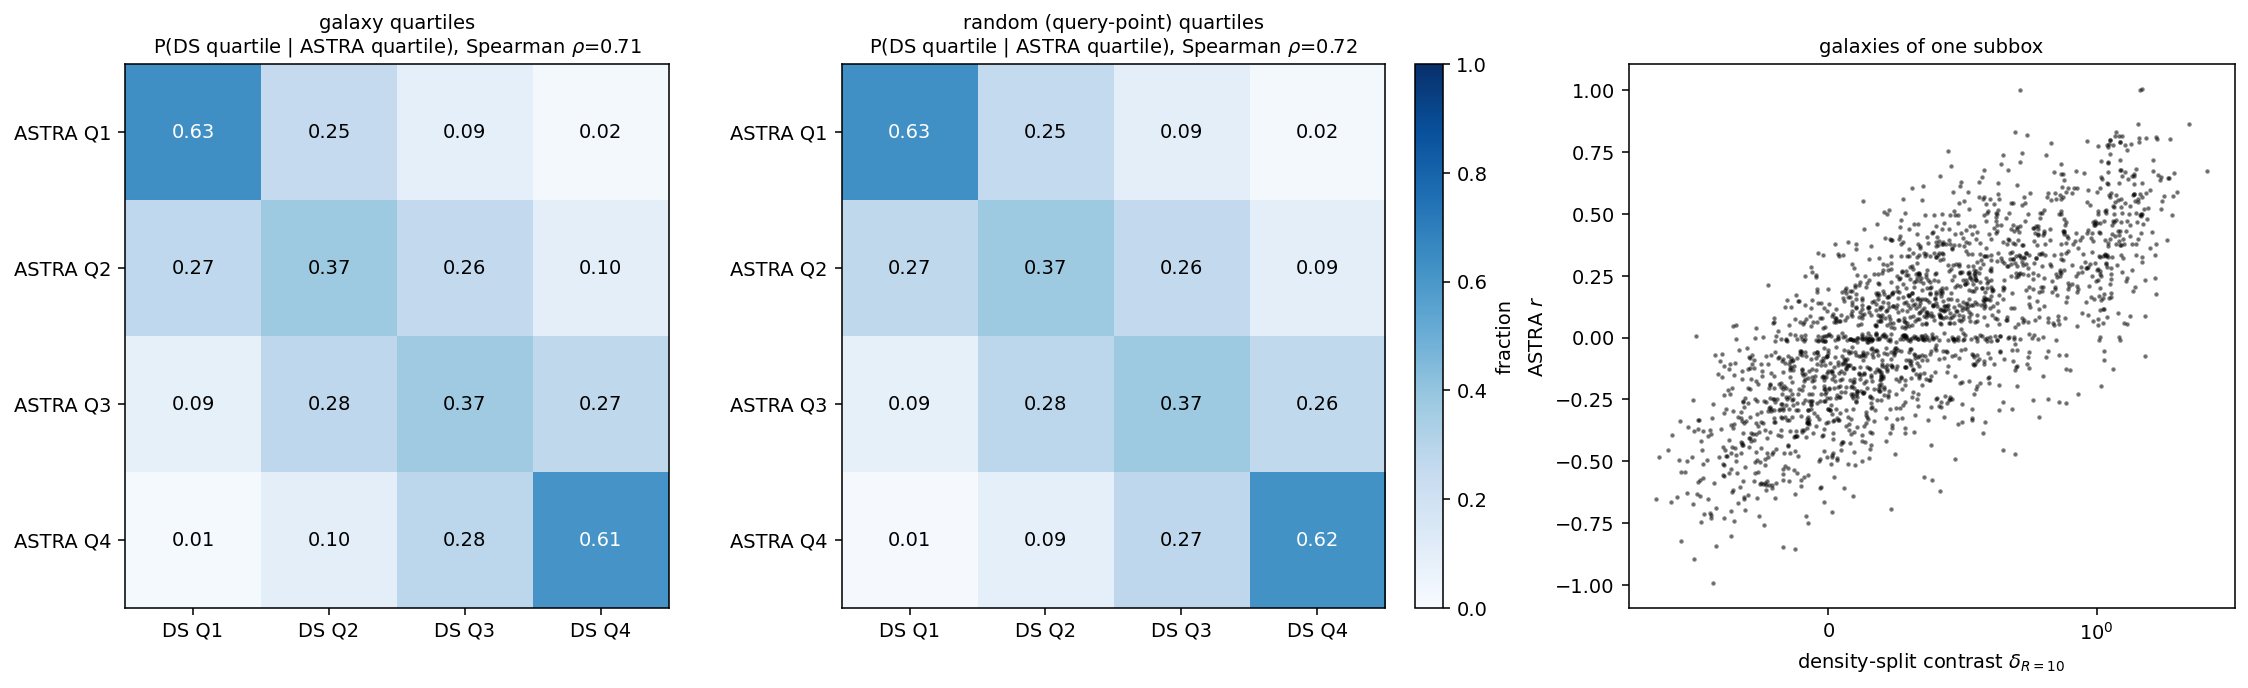
\includegraphics[width=0.95\textwidth]{v2_environment.png}
\caption{Environnements ASTRA et density split sur le catalogue fiduciel (\texttt{c000}, \texttt{hod239}, ligne de visée $z$). Gauche, milieu : probabilité qu'un point d'un quartile ASTRA donné tombe dans chaque quartile du density split, pour les galaxies et les points aléatoires (moyenne sur 64 sous-volumes). Droite : $r$ d'ASTRA en fonction du contraste de densité lissé pour un échantillon de galaxies (léger décalage vertical aléatoire ajouté au $r$ discret).}
\label{fig:env}
\end{figure*}

\begin{figure*}[!tp]
\centering
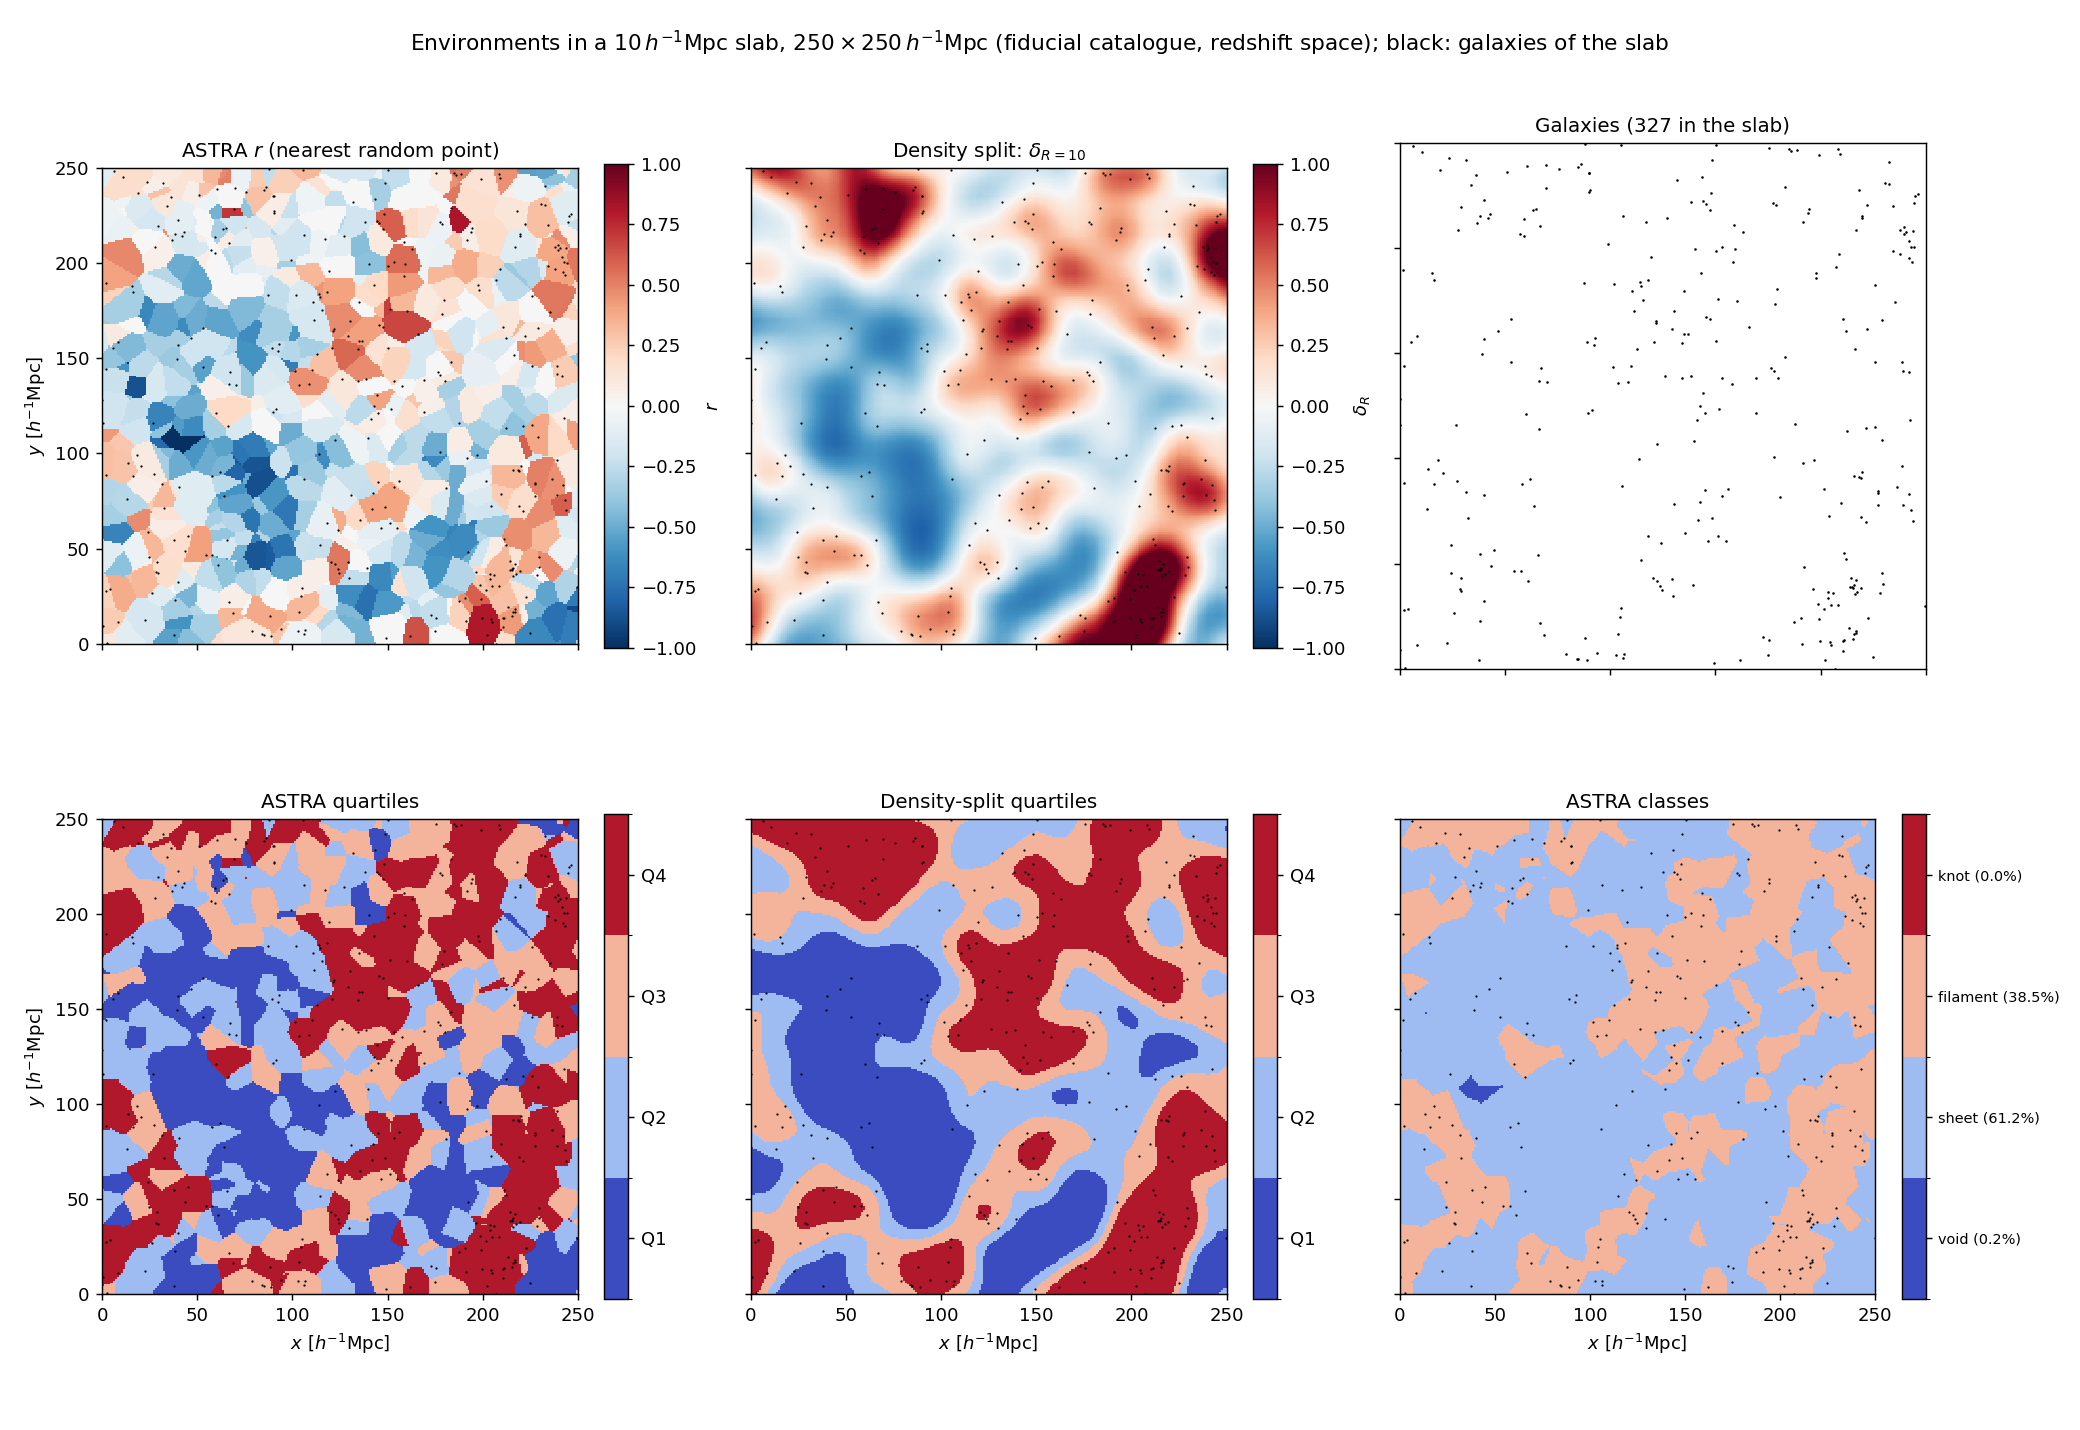
\includegraphics[width=\textwidth]{env_maps.png}
\caption{Environnements dans une tranche de $10\Mpch$ de $250\times250\Mpch$ du catalogue fiduciel, représentés par des régions remplies : chaque pixel prend la valeur ASTRA $r$, le quartile ou la classe du point aléatoire le plus proche (gauche, en bas à droite), ou le contraste de densité lissé et son quartile (centre) ; points noirs : galaxies de la tranche. ASTRA définit les environnements cellule par cellule, à l'échelle des voisins de Delaunay, alors que le density split les définit sur un champ lisse ; les classes ASTRA sont dominées par les feuillets et les filaments.}
\label{fig:map}
\end{figure*}

\begin{figure*}[!tp]
\centering
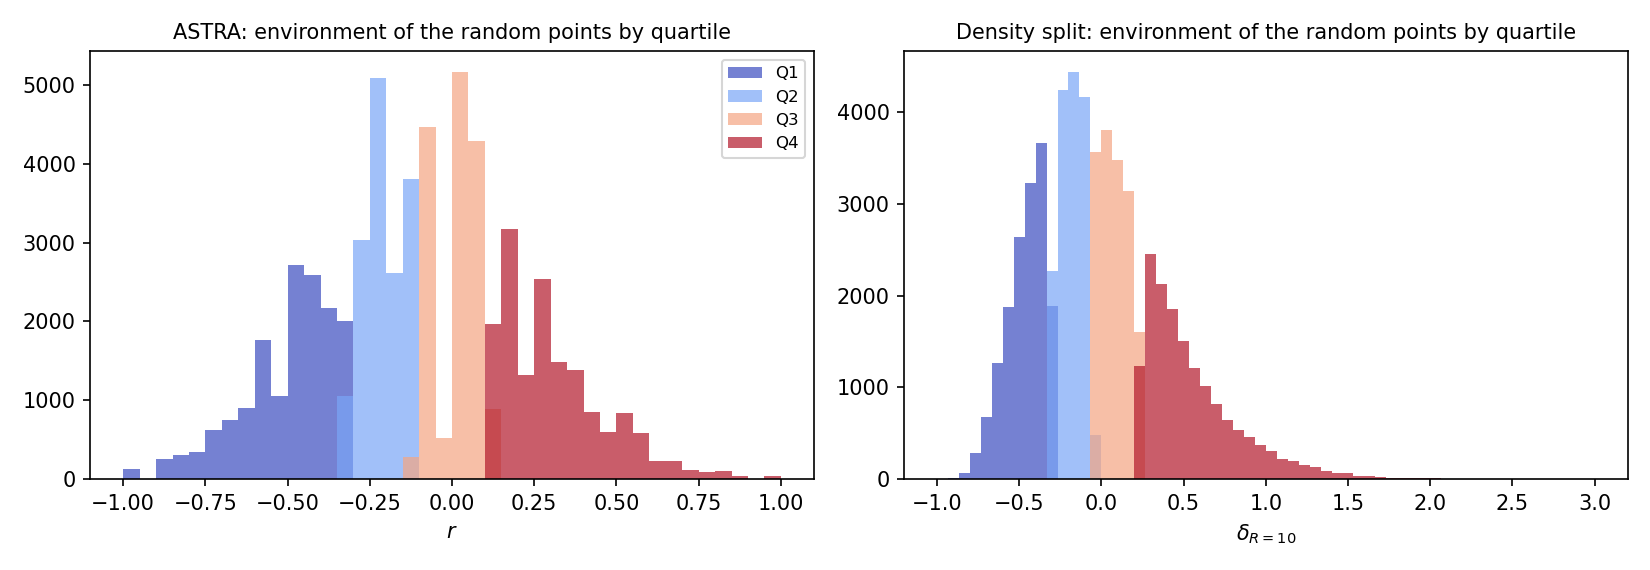
\includegraphics[width=0.85\textwidth]{v2_env_hist.png}
\caption{Distribution de l'environnement des points aléatoires par quartile : $r$ d'ASTRA (gauche, valeurs discrètes) et $\delta_R$ du density split (droite).}
\label{fig:envhist}
\end{figure*}

\begin{figure*}[!tp]
\centering
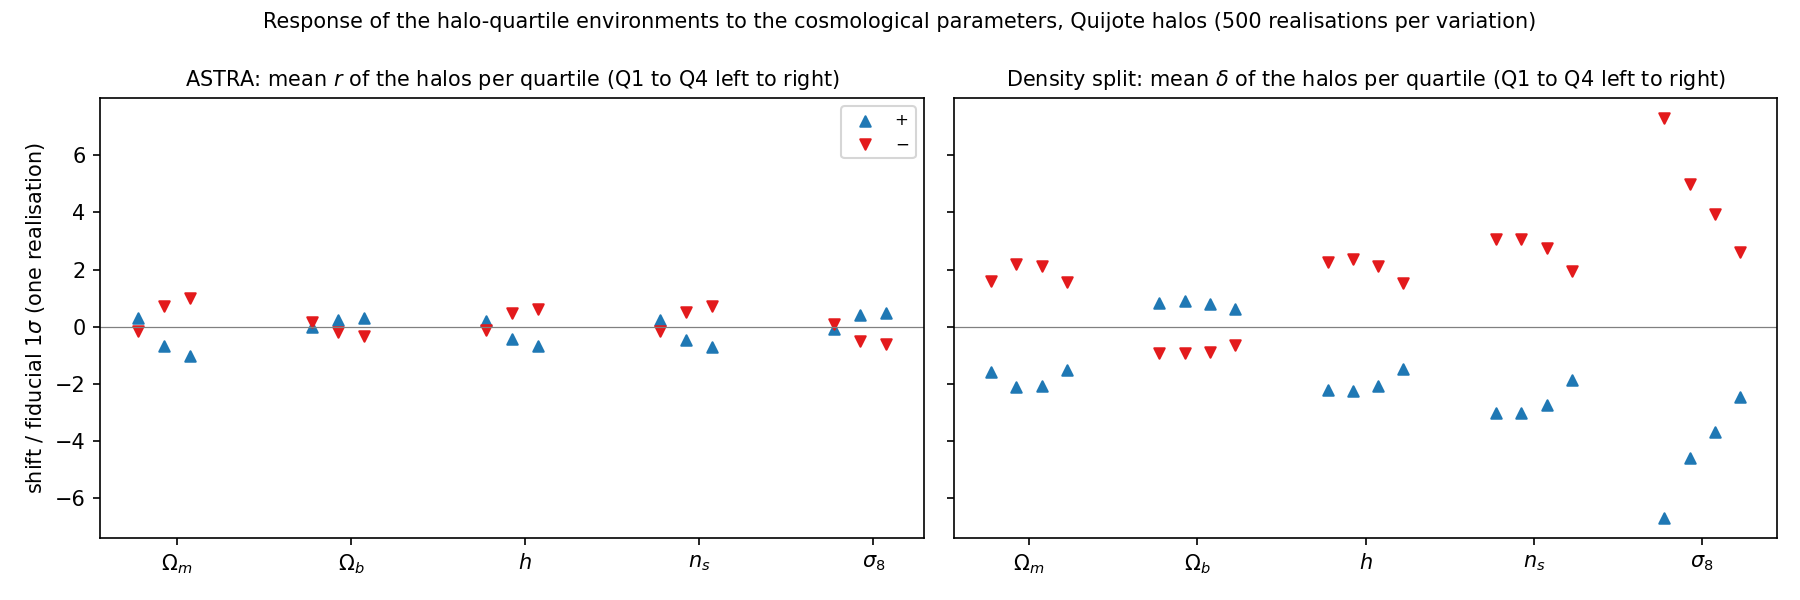
\includegraphics[width=\textwidth]{v2_response.png}
\caption{Décalage de l'environnement moyen de chaque quartile de halos (Q1 à Q4 de gauche à droite) pour les variations $+$ (bleu) et $-$ (rouge) de chaque paramètre, Quijote, en unités de la dispersion d'une réalisation. Gauche : $r$ d'ASTRA ; droite : $\delta_R$ du density split.}
\label{fig:response}
\end{figure*}

